\documentclass[letterpaper,twoside]{article}

\newcommand{\productName}{Atlas}
\newcommand{\productTeaser}{Multi-sensor Datalogger Board}
\newcommand{\companyName}{Aerodyne Labs}
\newcommand{\contactAddress}{sales@aerodynelabs.com}

\usepackage{geometry}
\setlength{\oddsidemargin}{15.5pt} 
\setlength{\evensidemargin}{15.5pt}

\usepackage{multicol}
\usepackage{mdwlist}
\usepackage{url}
\usepackage{graphicx}

\usepackage{fancyhdr}
\pagestyle{fancy}
\setlength{\headheight}{18pt}
% Create custom page style
\fancyhf{} % Clear defaults
\fancyhead[LE,RO]{\textbf{\Large{\productName}}}
\fancyhead[RE,LO]{\Large{\companyName}}
\fancyfoot[C]{\thepage}
\fancyfoot[LE,RO]{\contactAddress}
\fancyfoot[RE,LO]{\copyright \the\year \companyName}
\renewcommand{\headrulewidth}{2pt}
\renewcommand{\footrulewidth}{1pt}
% Override plan page style
\fancypagestyle{plain}{%
\fancyhf{} % Clear defaults
\fancyfoot[C]{\thepage}
\fancyfoot[LE,RO]{\contactAddress}
\fancyfoot[RE,LO]{\copyright \the\year \companyName}
\renewcommand{\headrulewidth}{0pt}
\renewcommand{\footrulewidth}{1pt}
}

\begin{document}

\thispagestyle{plain} % Kill header on first page
\textsf{\textbf{\Large{\companyName}}}\\
\rule{\linewidth}{2pt}
\vspace{8pt}
\par\textsf{\textbf{\Huge{\productName}}}
\vspace{16pt}
\par\textsf{\textbf{\Large{\productTeaser}}}
\vspace{8pt}\\
\rule{\linewidth}{1pt}
\vspace{8pt}

\begin{multicols}{2}

\section*{General Description}
Atlas is a shield that is designed to plug into the STMicroelectronics Nucleo boards as an add on shield.  The shield was designed and tested to work with the Nucleo F401RE development board which features a STM32F401 processor at 84 MHz based on the Cortex M4 Arm processor core.  This board also features Arduino compatible headers to allow additional expansion to existing Arduino shields.  The shield has an on board GPS, temperature, humidity, pressure and 9-DOF IMU sensor on board.  A micro SD card holder allows for data logging on the shield and xBee and RFD900 connectors allows for transmitting the data wirelessly.  
\ \\ \ \\

%\begin{wrapfigure}{R}{0.45\textwidth}
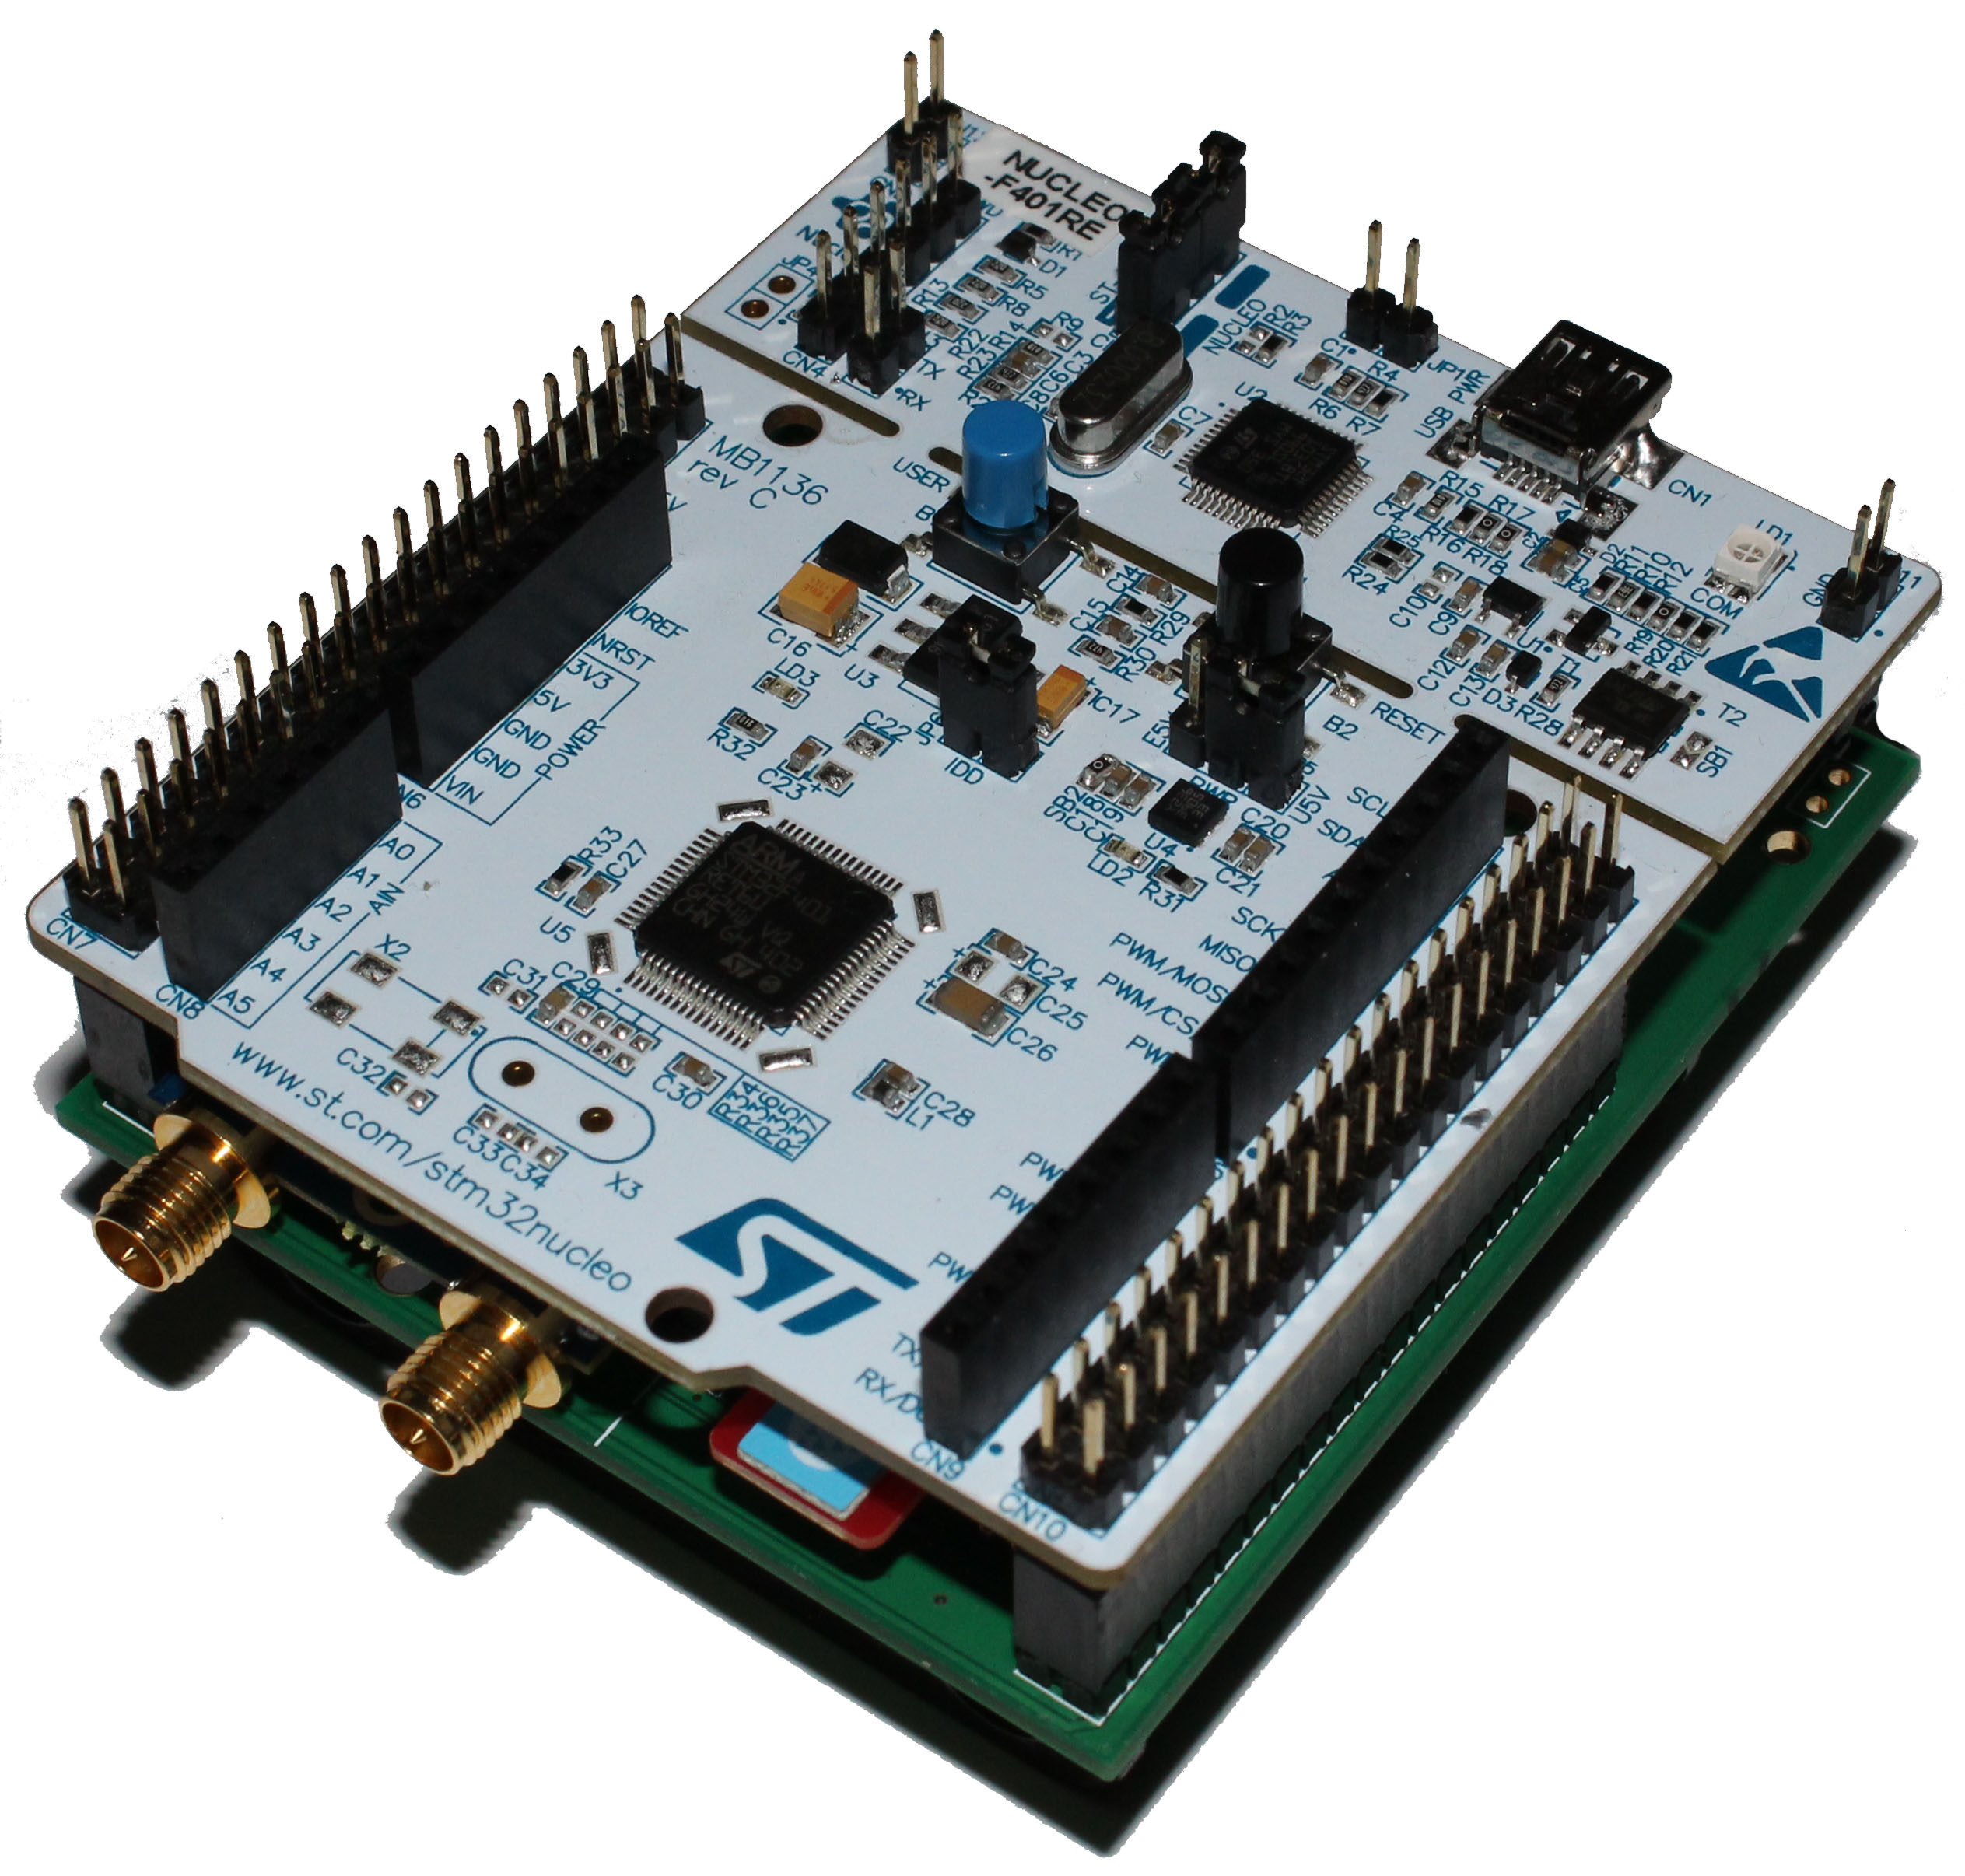
\includegraphics[scale=.06]{images/Atlas.jpg}
%\end{wrapfigure}


\vfill
\columnbreak

\section*{Features}
\begin{itemize*}
	\item 84 MHz Cortex M4 Arm processor
	\item Easy programming using the MBED online IDE 
	\item Single chip 9-DOF Inertial Measurement Unit
	\item Up to 40 Hz output GPS suitable for high altitude use
	\item Barometric pressure sensor with 10 cm resolution
	\item High resolution temperature and humidity sensor
	\item Flexible power system
	\item On-board removable micro SD card
\end{itemize*}

\end{multicols}

\newpage

\tableofcontents

\section{Overview}
Where is everything on this thing

\section{Quick Start}
Use of the Atlas shield is fairly straightforward.  Before attaching the board to a Nucleo F401RE board, make sure the following are done first.
\begin{itemize*}
	\item Ensure a micro SD card is inserted into the board
	\item Plug in either a RFD900 \emph{or} xBee unit to the appropriate header\footnote{Inserting both an xBee unit and RFD900 will cause problems and may damage the shield}
	\item If using AA batteries, make sure the remove before flight pin is inserted
	\item If using AA batteries, makes sure a fresh set of batteries is installed\footnote{Aerodyne labs recommends AA Lithium Batteries if using the RFD900 or xBee option}
\end{itemize*}

Simply plug the shield into the Nucleo F401RE board.  The shield is designed and only plugs in to the bottom of the Nucleo board unlike most shields which plug on the top.  

How to make this thing do its thing quickly so you can eat a sammich

\section{Programming and Firmware Instructions}
How to set this thing up, programming with mbed and other software...stuff

\section{Hardware Specifications and Information}
More detailed specifications and additional information about this device

\section{Hints and Tips}
Additional hints and tips for using the board including some tips for using it for high altitude ballooning.

\appendix
\newpage
\section*{Troubleshooting}
\begin{center}
\begin{tabular}{l | p{0.65\textwidth}}
Symptom & Solutions \\
\hline
Symptom number one &%
$\bullet$ Solution number one\newline
$\bullet$ Solution number two\\
Symptom number two &%
Solution number one\newline
Solution number two
\end{tabular}
\end{center}

\section*{Customer Support}
If you require support for your device, please first read the troubleshooting section of this manual. If you are unable to resolve the problem please check the product page at \url{http://www.aerodynelabs.com/products/atlas} for any updated documentation or software. If your problem persists, please contact \url{support@aerodynelabs.com} for further help.

\end{document}